\large
Stonehenge: $\sim$3100 - 2075 a.C.
\begin{center}
	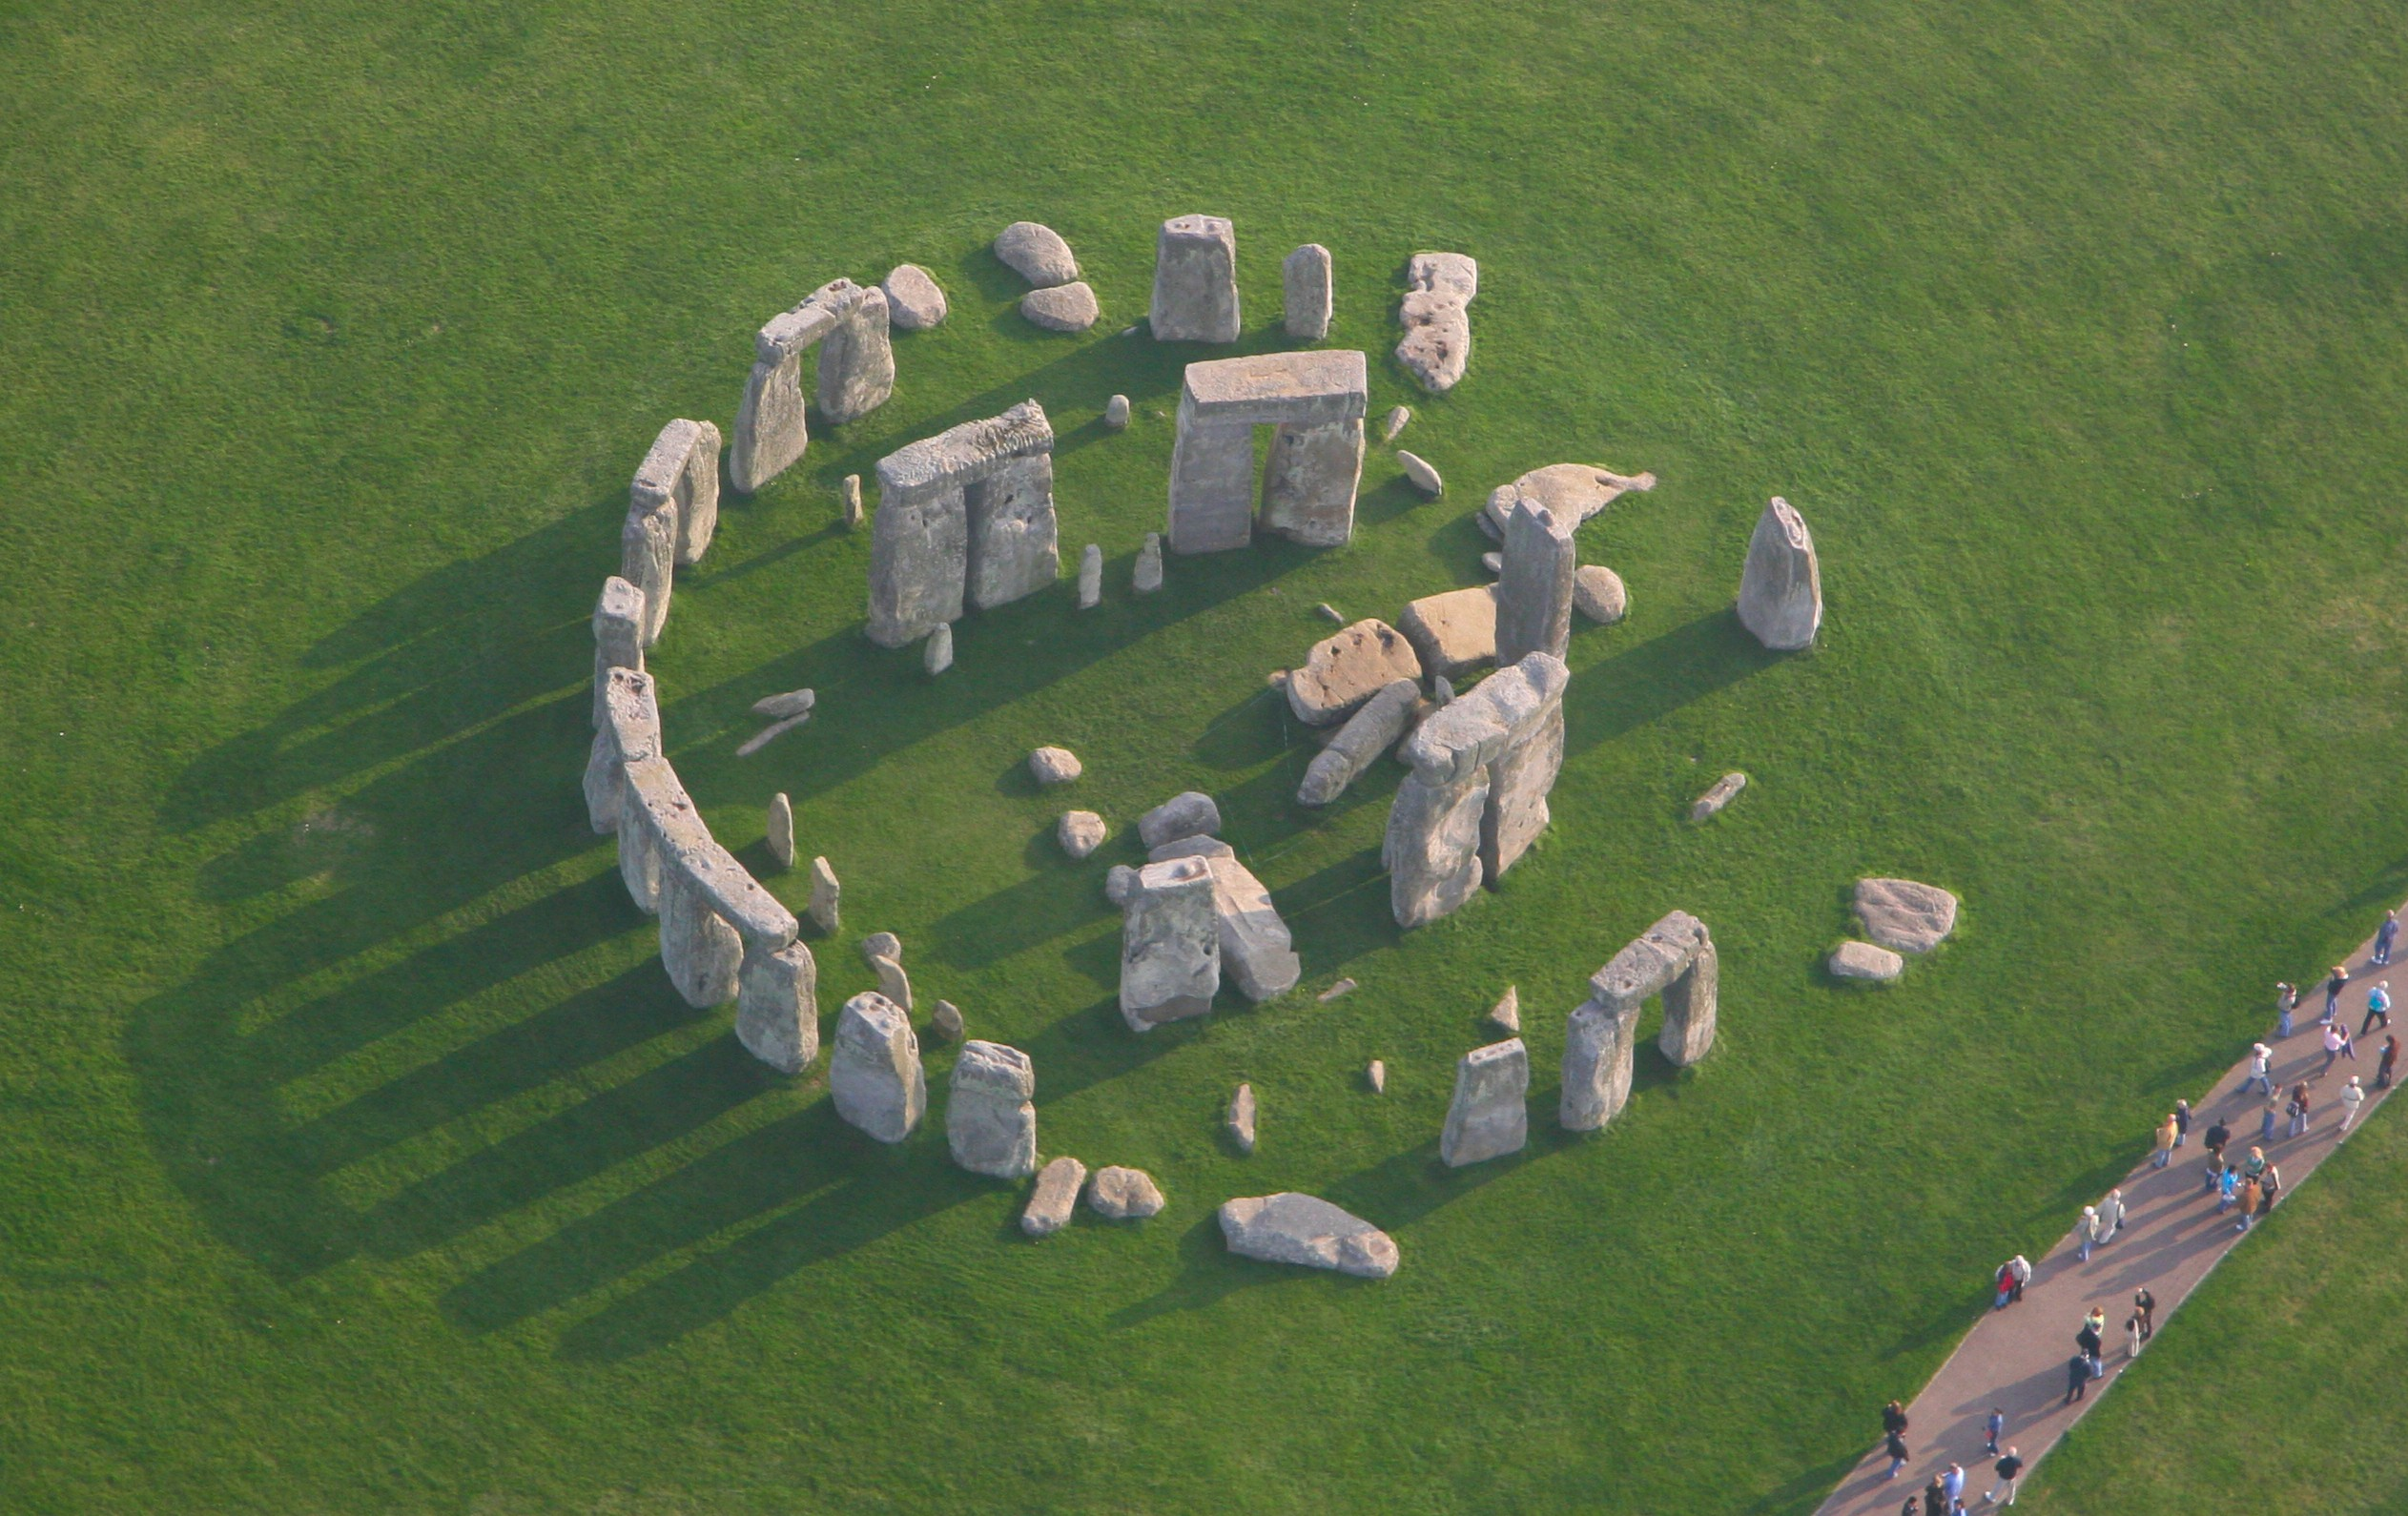
\includegraphics[height=.75\textheight]{./IMG/valuable_europe_265732.jpg}
\end{center}

\vfill
\pagebreak

\begin{multicols}{2}
	
	Relógio de sol: $\sim$1500 a.C.
	\begin{center}
		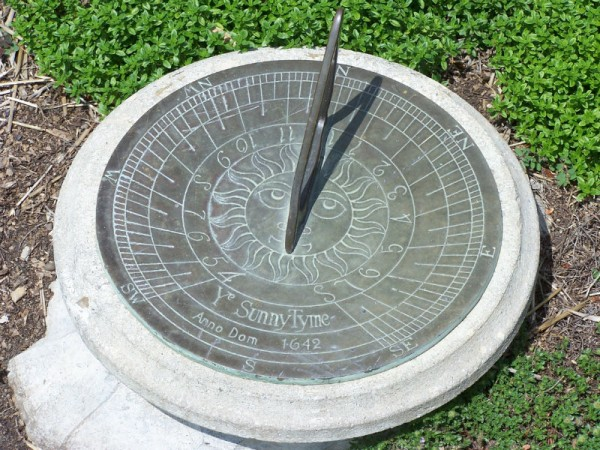
\includegraphics[width=\linewidth]{./IMG/Tempo-Relogio-de-Sol-600x450.jpg}
	\end{center}

\vfill\null
\columnbreak

Clepsidra: $\sim$1400 a.C.
	\begin{center}
	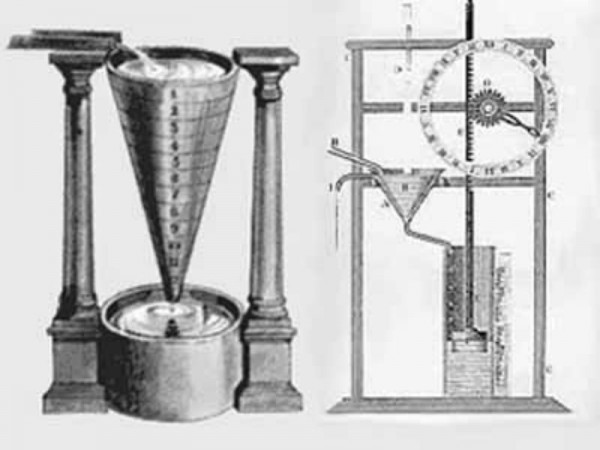
\includegraphics[width=\linewidth]{./IMG/Tempo-Clepsidra-600x450.jpg}
\end{center}

\vfill
\pagebreak
\end{multicols}

\begin{multicols}{3}

Anticítera: $\sim$séc 1 a.C.

		\begin{center}
	\includegraphics[width=\linewidth]{./IMG/NAMA_Machine_d'Anticythère_1.jpg}
\end{center}

\vfill\null
\columnbreak

\begin{center}
	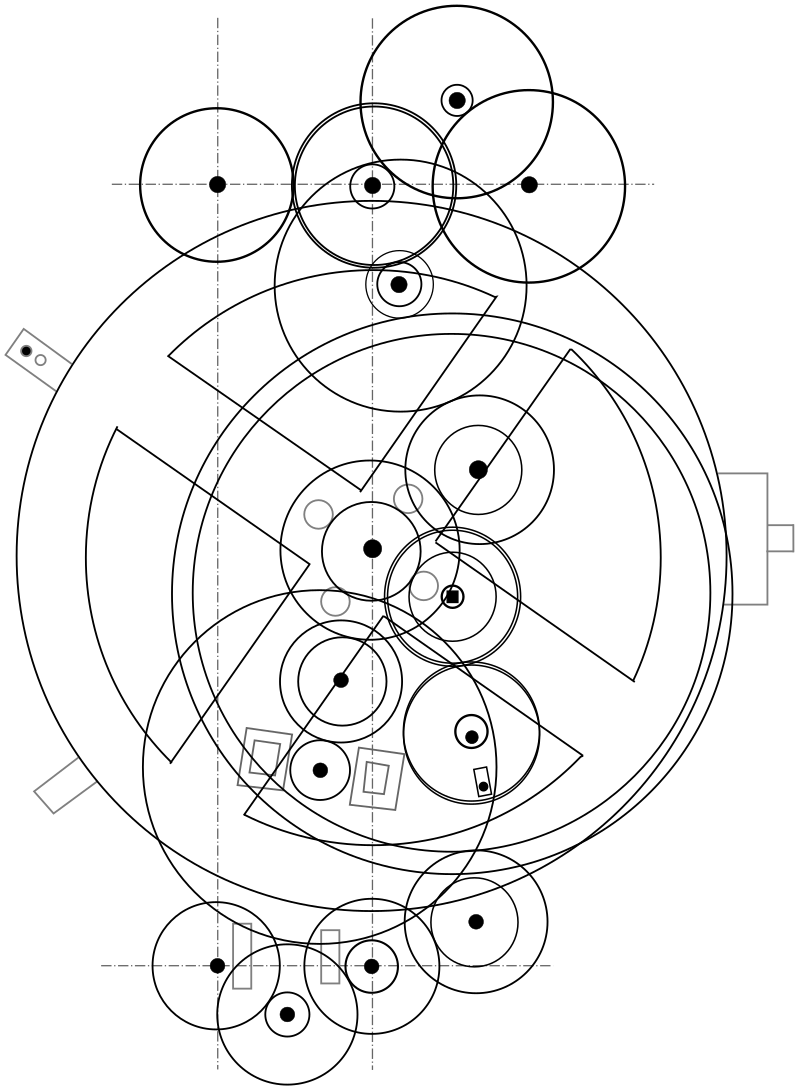
\includegraphics[width=\linewidth]{./IMG/800px-Antikythera_mechanism.svg}
\end{center}

\vfill\null
\columnbreak

\begin{center}
	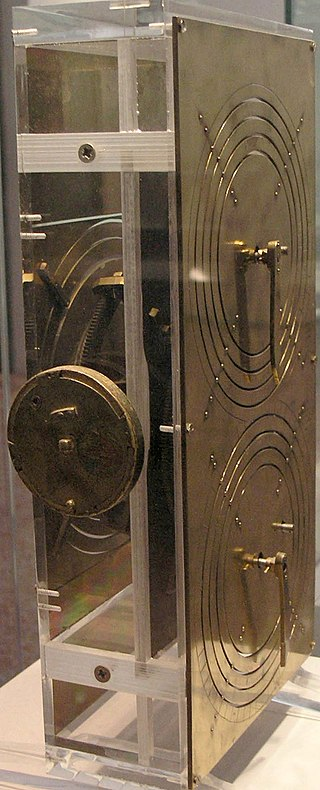
\includegraphics[width=.9\linewidth,height=\textheight]{./IMG/Anticythere.jpg}
\end{center}

\vfill
\pagebreak

Ampulheta: $\sim$sec. 7.
	\begin{center}
	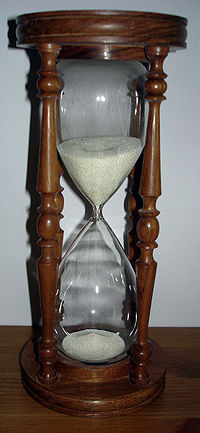
\includegraphics[height=.9\textheight]{./IMG/200px-Wooden_hourglass.jpg}
\end{center}

\vfill
\columnbreak

Relógio de vela: $\sim$sec. 8.
	\begin{center}
	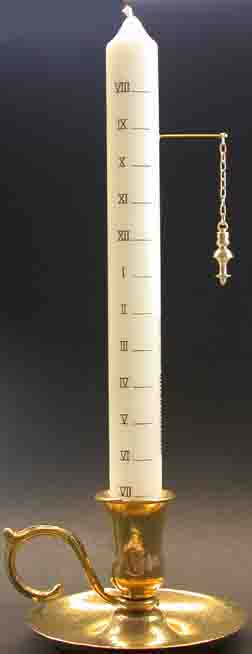
\includegraphics[height=.9\textheight]{./IMG/aeb6915395e4f1a99f80b6f692a88e22.jpg}
\end{center}

\vfill
\columnbreak

Relógio de pêndulo\\(Christiaan Huygens):  1656.

	\begin{center}
	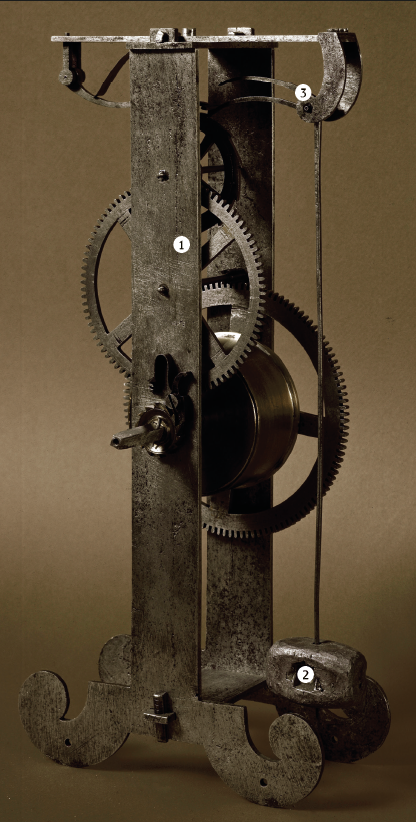
\includegraphics[height=.8\textheight]{./IMG/g8.png}
\end{center}
\end{multicols}
\vfill
\pagebreak

\begin{multicols}{2}

Relógio de quartzo (Warren Marrison): 1955.

\begin{center}
	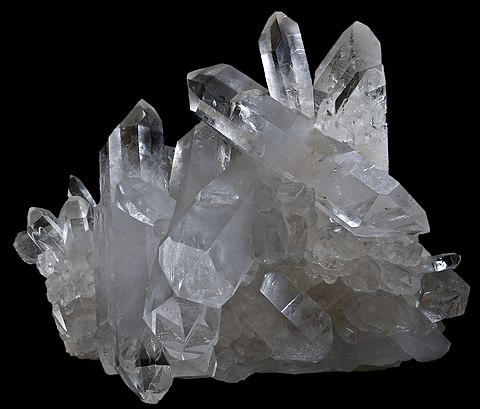
\includegraphics[height=.8\textheight]{./IMG/Quartz_Brésil.jpg}
\end{center}

\vfill
\columnbreak

\begin{center}
	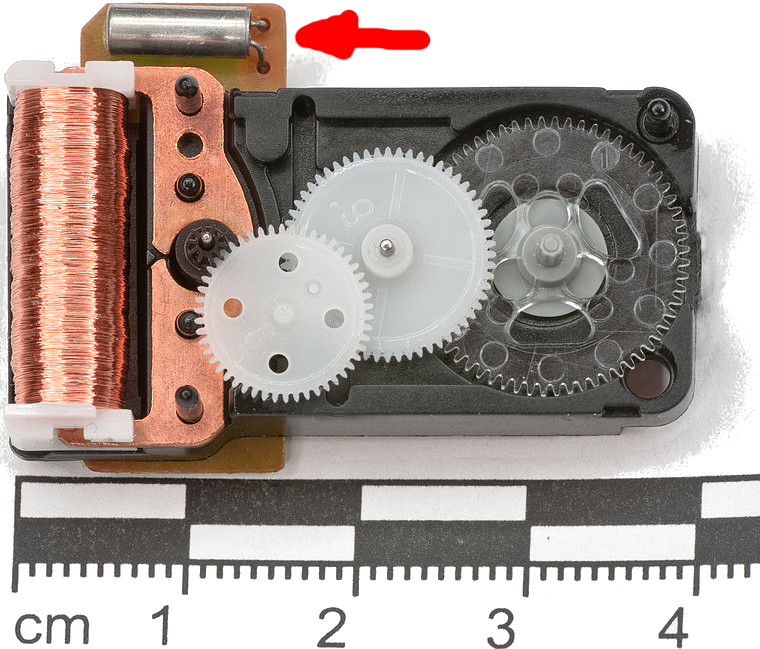
\includegraphics[width=\linewidth]{./IMG/800px-Quartz_Clockwork_(disassembled).jpg}
\end{center}

\vfill\null
\columnbreak

Relógio atômico: 1955.
	\begin{center}
	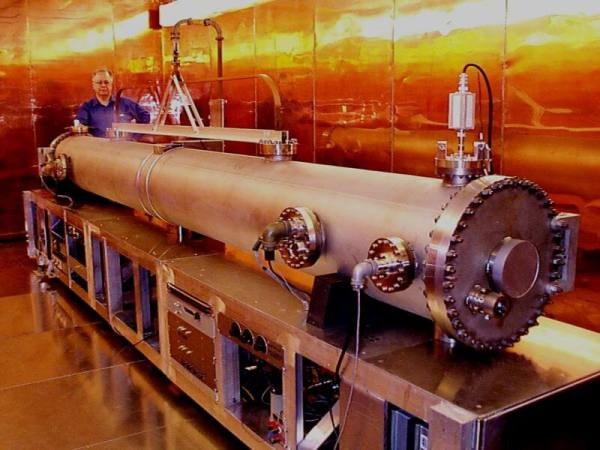
\includegraphics[width=\linewidth]{./IMG/Tempo-Relogio-Atomico-600x450.jpg}
\end{center}

\vfill
\columnbreak

\begin{center}
	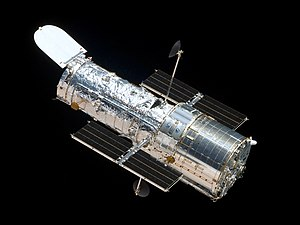
\includegraphics[width=\linewidth]{./IMG/HST-SM4.jpeg}
\end{center}
\end{multicols}

\vfill\null
\pagebreak
